\documentclass[page number]{beamer}
\usetheme[sectionpage=none,numbering=fraction,progressbar=foot]{metropolis}

\usepackage{pgf,tikz}
\usetikzlibrary{arrows}
\usetikzlibrary{positioning,shapes,fit,automata}
\usepackage{xcolor}
\usepackage{amssymb}
\usepackage{amsmath}

\makeatletter
\makeatother

\setcounter{tocdepth}{1} % remove subsection from table of contents

% colors
\definecolor{mDarkRed}{HTML}{6F1616}
\definecolor{mDarkGreen}{HTML}{106235}
\definecolor{mTeal}{HTML}{112233}
\definecolor{mBlack}{HTML}{000000}
\setbeamercolor{normal text}{fg=mTeal}
\setbeamercolor{alerted text}{fg=mDarkRed}
\setbeamercolor{example text}{fg=mDarkGreen}
\setbeamercolor{title separator}{fg=purple,bg=mBlack}

\def\outline{
  \begin{frame}[plain,noframenumbering]
    \frametitle{Outline}
    \tableofcontents[currentsection]
  \end{frame}
}


\begin{document}
\title{Undecidable problems about timed automata\\ Olivier Finkel}

\author{Aur\`ele Barri\`ere \& Joshua Peignier}

\date{\textit{ENS Rennes}
  \vfill
  \textbf{January 9, 2019}}

\def\outline{
  \begin{frame}[plain,noframenumbering]
    \frametitle{Outline}
    \tableofcontents[currentsection]
  \end{frame}
}

\begin{frame}[plain,noframenumbering]
  \vspace{-2cm}
  \maketitle
  \vspace{-4cm}
\end{frame}

\begin{frame}{Timed Automatas}

  \dots
  
\end{frame}

\begin{frame}{Proof}

  \begin{block}{Theorem}
    The following problems are undecidable.
  \end{block}

  \begin{alertblock}{Equivalence with a deterministic timed automaton}
    \begin{itemize}
	\item \textbf{Input} : a timed automaton $\mathcal{A}$.
	\item \textbf{Output} : yes if there exists a deterministic timed automaton $\mathcal{B}$ such that $\mathcal{L}(\mathcal{A}) = \mathcal{L}(\mathcal{B})$, else no.
    \end{itemize}
  \end{alertblock}
  
    \begin{alertblock}{Acceptation of the complement}
    \begin{itemize}
	\item \textbf{Input} : a timed automaton $\mathcal{A}$.
	\item \textbf{Output} : yes if there exists a timed automaton $\mathcal{B}$ such that $\mathcal{L}(\mathcal{A})^c = \mathcal{L}(\mathcal{B})$, else no.
    \end{itemize}
  \end{alertblock}

\end{frame}


\begin{frame}{Proof}

   \begin{block}{Notation}
    Let $A$ be the language of words of the form $t_1 a \dots t_n a$ such that there exists a pair of $a$ separated by a time distance $1$:
$$\exists i,j [\![1,n]\!], i < j  \land  t_{i+1} + \dots + t_j = 1$$
  \end{block}

  \begin{block}{Property}
    The language $A$ is timed regular.\\
    The language $A^c$ is not timed regular.
  \end{block}

  \begin{block}{Proof idea}
    If there existed a timed automaton accepting $A^c$, it would need an unbounded number of clocks.\\
    \textbf{maybe draw the automaton for $A$ ?}
  \end{block}

\end{frame}


\begin{frame}{Proof}

	\begin{block}{Notation}
	    $\Sigma$ is an alphabet containing $a$ ; $c$ is a letter not in $\Sigma$. $\Gamma = \Sigma \cup \{c\}$.
  	\end{block}

	\begin{block}{Goal}
		$L$ is a timed regular language over $(\mathbb{R}\times\Sigma)^*$, and an input of the universability problem. Build the reduction to equivalence with a deterministic timed automaton and to acceptation of the complement.\\
  	\end{block}

	\begin{block}{Notation}
		\begin{itemize}
			\item $\mathcal{L}_1 = L.(\mathbb{R} \times \{c\}).(\mathbb{R}\times\Sigma)^*$
			\item $\mathcal{L}_2$: set of words over $\Sigma$ with no $c$ or at least two $c$.
			\item $\mathcal{L}_3 = (\mathbb{R}\times\Sigma)^*.(\mathbb{R} \times \{c\}).A$
		\end{itemize}
  	\end{block}

\end{frame}


\begin{frame}{Proof}

	\begin{block}{Notation}
		$\mathcal{L} = \mathcal{L}_1 \cup \mathcal{L}_2 \cup \mathcal{L}_3$ is the input to equivalence with a deterministic timed automaton and acceptation of the complement, built from $L$.
	\end{block}

	\begin{block}{Property}
		$\mathcal{L} = \mathcal{L}_1 \cup \mathcal{L}_2 \cup \mathcal{L}_3$ is timed regular, since $L$ and $A$ are timed regular.
	\end{block}

	\begin{block}{Lemma}
		If $L$ is universal, then $\mathcal{L}$ is accepted by a deterministic timed automaton, and $\mathcal{L}^c$ is accepted by a timed automaton.
	\end{block}

	\begin{block}{Proof}
		Easy: if $L = (\mathbb{R}\times\Sigma)^*$, then $\mathcal{L} = (\mathbb{R}\times\Gamma)^*$ and $\mathcal{L}^c = \emptyset$.
	\end{block}

	
\end{frame}


\begin{frame}{Proof}

	\begin{block}{Lemma}
		If $L \subsetneq (\mathbb{R}\times\Sigma)^*$, then $\mathcal{L}^c$ is not timed regular.
	\end{block}
	
	\begin{block}{Proof}
	Let $u = t_1 a_1 \dots t_n a_n \not\in L$, and $x \in (\mathbb{R}\times\Sigma)^*$. Then $u 1 c x \in \mathcal{L}$ iff $x \in A$. Thus, $u 1 c x \in \mathcal{L}^c$ iff $x \in A^c$.\\
	\textbf{Proof of not-regularity of $\mathcal{L}^c$: similar to the one of $x \in A^c$, which is not detailed.}
	\end{block}

\end{frame}


\begin{frame}{Known Results on Timed Automata - Clock Minimization}

  \begin{alertblock}{Minimization of the number of clocks}
    Given $\mathcal{A}$ a timed automaton with $n$ clocks, is there an automaton $\mathcal{B}$ with $n-1$ clocks such that $\mathcal{L(B)=L(A)}$? If so, construct $\mathcal{B}$.\\
    This problem is known to be \textbf{undecidable}.
  \end{alertblock}
  \vfill
  \begin{exampleblock}{What if we don't ask for a witness?}
    Simply answer Yes or No if the number of clocks can be reduced (decision problem).
  \end{exampleblock}
    
\end{frame}

\begin{frame}{Back to clock minimization}
  
  \begin{alertblock}{Undecidable problem}
    Given $\mathcal{A}$ a timed automaton with $n$ clocks, is there an automaton $\mathcal{B}$ with $n-1$ clocks such that $\mathcal{L(B)=L(A)}$?
  \end{alertblock}

  Give idea of the proof.
  
\end{frame}

\begin{frame}{Shuffle operation}
  \begin{block}{Shuffling}
    $$x\bowtie y = \{x_1 . y_1 . \dots . x_n . y_n~|~x=x_1\dots x_n\text{ and }y=y_1\dots y_n\}$$
  \end{block}

  \begin{block}{Shuffling Sets}
    Let $R_1, R_2\subseteq M$.
    $$R_1\bowtie R_2 = \{x\bowtie y~|~x\in R_1~\text{and}~y\in R_2\}$$
  \end{block}

  \begin{exampleblock}{Shuffling regular untimed languages}
    The class of regular untimed languages is closed under shuffle.\\
    What about timed languages?
  \end{exampleblock}
  
\end{frame}


\begin{frame}{Shuffling timed languages}
  \begin{alertblock}{Shuffling timed regular languages is not always regular}
  \end{alertblock}

  $R_1=\{t_1 . a . 1 . a . t_2 . a~|~t_1+t_2 = 1\}$.
  Regular language.

  \begin{figure}
    \centering
    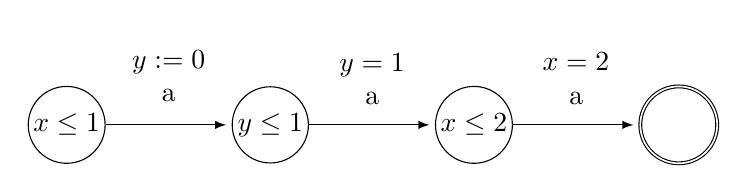
\begin{tikzpicture}[%
        every node/.style={circle, minimum size=4pt,minimum height=4pt, inner sep=1pt, align=center},
        shorten >=2pt,
        node distance=1.6cm, >=latex
      ]
      \node [] (s0) [draw] {$x\leq 1$};
      \node [] (s1) [draw, right=of s0] {$y\leq 1$};
      \node [] (s2) [draw, right=of s1] {$x\leq 2$};
      \node [] (s3) [draw, accepting, right=of s2] {\phantom{$x\leq 2$}};
      \path [draw] (s0) edge[->,above]  node {$y:=0$\\a} (s1)
      (s1) edge[->,above]  node {$y=1$\\a} (s2)
      (s2) edge[->,above]  node {$x=2$\\a} (s3);
    \end{tikzpicture}
  \end{figure}


  $R_2=\{1 . b . s . b ~|~ s\in\mathbb{R}\}$. Regular.

  Prove that $R_1\bowtie R_2$ is not timed regular.

  If it was, then $\{t_1.a.\mathbf{1.b.s.b}.1.a.t_2.a~|~t_1+t_2=1\}$ would be too.
\end{frame}

\begin{frame}{Shuffling timed language}
  Assume we have an automata for $\{t_1.a.\mathbf{1.b.s.b}.1.a.t_2.a~|~t_1+t_2=1\}$.
  
  After reading $t_1.a.\mathbf{1.b.s.b}.1.a$, the clocks can either be
  \begin{itemize}
  \item $t_1+s=2$
  \item $s+2$
  \item $s+1$
  \item 1
  \end{itemize}
  
  With any of these values, we can't derive a test to accept $t_2$ such that $t_1+t_2=1$.
  
  \begin{exampleblock}{Theorem}
    It is undecidable to determine whether the shuffle of two timed regular languages is timed regular.\\
    Reduction from the universality problem.
  \end{exampleblock}
\end{frame}

\begin{frame}{Corollaries}
  \begin{block}{Bounded Ressources}
    $TA(n,K)$ Timed automata with at most $n$ clocks and constants are $\leq K$.\\
    \begin{itemize}
    \item Given $\mathcal{A,B},n,K$, decide if there is $\mathcal{C} TA(n,K)$ such that $L(\mathcal{C})=L(\mathcal{A})\bowtie L(\mathcal{B})$. \textbf{Undecidable}.
    \item Given $\mathcal{A,B},n$, decide if there is $\mathcal{C}$ with at most $n$ clocks such that $L(\mathcal{C})=L(\mathcal{A})\bowtie L(\mathcal{B})$. \textbf{Undecidable}.
    \item Given $\mathcal{A,B},n,K$, decide if there is $\mathcal{C} TA$ such that $L(\mathcal{C})=L(\mathcal{A})\bowtie L(\mathcal{B})$. \textbf{Undecidable}.
    \end{itemize}
  \end{block}
  \vfill
  
    
\end{frame}

\begin{frame}{Timed B\"uchi automata}
  \begin{block}{Definition}
    Accept infinite words of $(\mathbb{R}\times\Sigma)^\omega$.
  \end{block}
  \vfill
  \begin{alertblock}{Known Result}
    The universality problem for Timed B\"uchi automata is $\Pi^1_1$-hard.
  \end{alertblock}
  \vfill
  \begin{exampleblock}{Theorems}
    Given Timed B\"uchi Automata (TBA) $\mathcal{A}$, decide if
    \begin{itemize}
    \item Its language is accepted by a deterministic TBA
    \item Its complementation is accepted by a TBA
    \end{itemize}
    Both problems are \textit{highly undecidable}. $\Pi^1_1$-hard.
  \end{exampleblock}

\end{frame}

\begin{frame}{Conclusion}
  \begin{block}{Overview}
    \begin{itemize}
    \item FORMATS'06
    \item 52 citations
    \end{itemize}
  \end{block}
  \vfill
  \begin{exampleblock}{Contribution}
    \begin{itemize}
    \item Solved several open problems
    \item Proof strategy that works for many problems
    \item Re-proved some known results
    \end{itemize}
  \end{exampleblock}
\end{frame}


\end{document}
